% ============================================================
% Rapport Technique --- Rapport 2
% An Agentic Framework for IaC Misconfiguration Analysis
% and Remediation
%
% Ahmedou Yahye Kheyri
% Supervised by: Hala Bezine
% Faculté des Sciences de Sfax --- Master MRSI
% 2025--2026
% ============================================================

\documentclass[12pt, a4paper]{report}

% ---- Encoding & Language ----
\usepackage[utf8]{inputenc}
\usepackage[T1]{fontenc}
\usepackage[english]{babel}

% ---- Layout ----
\usepackage[
  top=2.5cm, bottom=2.5cm,
  left=3cm,  right=2.5cm
]{geometry}
\usepackage{setspace}
\onehalfspacing
\setlength{\parindent}{1.2em}
\setlength{\parskip}{0.4em}
\setlength{\headheight}{14pt}

% ---- Fonts ----
\usepackage{lmodern}
\usepackage{microtype}

% ---- Math ----
\usepackage{amsmath}
\usepackage{amssymb}

% ---- Graphics & Tables ----
\usepackage{graphicx}
\usepackage{float}
\usepackage{booktabs}
\usepackage{tabularx}
\usepackage{multirow}
\usepackage{longtable}
\usepackage{array}
\usepackage[table,xcdraw]{xcolor}

% ---- Code Listings ----
\usepackage{listings}
\usepackage{lstautogobble}

\definecolor{codegreen}{rgb}{0.0,0.5,0.0}
\definecolor{codegray}{rgb}{0.5,0.5,0.5}
\definecolor{codepurple}{rgb}{0.58,0,0.82}
\definecolor{backcolour}{rgb}{0.97,0.97,0.97}
\definecolor{codeblue}{rgb}{0.0,0.0,0.7}

\lstdefinestyle{iacstyle}{
  backgroundcolor=\color{backcolour},
  commentstyle=\color{codegreen}\itshape,
  keywordstyle=\color{codeblue}\bfseries,
  stringstyle=\color{codepurple},
  basicstyle=\ttfamily\small,
  breakatwhitespace=false,
  breaklines=true,
  captionpos=b,
  keepspaces=true,
  numbers=left,
  numbersep=6pt,
  numberstyle=\tiny\color{codegray},
  showspaces=false,
  showstringspaces=false,
  showtabs=false,
  tabsize=2,
  frame=single,
  rulecolor=\color{gray!40},
  autogobble=true
}
\lstset{style=iacstyle}

% ---- TikZ for architecture diagram ----
\usepackage{tikz}
\usetikzlibrary{shapes.geometric, arrows.meta, positioning, fit, backgrounds, calc}

% ---- PGFPlots for charts ----
\usepackage{pgfplots}
\pgfplotsset{compat=1.18}
\usepackage{pgfplotstable}

% ---- Colors ----
\definecolor{agentblue}{RGB}{70,130,180}
\definecolor{analyzergreen}{RGB}{60,160,90}
\definecolor{kbpurple}{RGB}{130,80,170}
\definecolor{generatororange}{RGB}{210,120,30}
\definecolor{validatorsalmon}{RGB}{200,80,60}
\definecolor{formatterpink}{RGB}{180,60,120}
\definecolor{lightgray}{RGB}{245,245,245}

% ---- Headers & Footers ----
\usepackage{fancyhdr}
\pagestyle{fancy}
\fancyhf{}
\fancyhead[L]{\small\leftmark}
\fancyhead[R]{\small\thepage}
\fancyfoot[C]{\small Ahmedou Yahye Kheyri --- Faculté des Sciences de Sfax}
\renewcommand{\headrulewidth}{0.4pt}
\renewcommand{\footrulewidth}{0.2pt}

% ---- Hyperlinks ----
\usepackage[
  colorlinks=true,
  linkcolor=blue!70!black,
  citecolor=blue!60!black,
  urlcolor=blue!80!black,
  bookmarks=true,
  bookmarksnumbered=true
]{hyperref}
\usepackage{url}

% ---- Bibliography ----
\usepackage[numbers,sort&compress]{natbib}
\bibliographystyle{IEEEtranN}

% ---- Caption ----
\usepackage[font=small,labelfont=bf]{caption}
\usepackage{subcaption}

% ---- Boxes & Environments ----
\usepackage{tcolorbox}
\tcbuselibrary{breakable, skins}

\newtcolorbox{researchbox}[1][]{
  colback=blue!5!white, colframe=blue!50!black,
  fonttitle=\bfseries, title={#1},
  breakable, enhanced
}

\newtcolorbox{definitionbox}[1][]{
  colback=green!5!white, colframe=green!50!black,
  fonttitle=\bfseries, title={#1},
  breakable, enhanced
}

% ---- Chapter style ----
\usepackage{titlesec}
\titleformat{\chapter}[display]
  {\normalfont\huge\bfseries\color{agentblue}}
  {\chaptertitlename\ \thechapter}{16pt}{\Huge}
\titlespacing*{\chapter}{0pt}{-10pt}{20pt}

% ---- Acronyms ----
\usepackage[acronym,toc]{glossaries}
\makeglossaries
\newacronym{iac}{IaC}{Infrastructure as Code}
\newacronym{llm}{LLM}{Large Language Model}
\newacronym{rag}{RAG}{Retrieval-Augmented Generation}
\newacronym{crag}{CRAG}{Corrective Retrieval-Augmented Generation}
\newacronym{cwe}{CWE}{Common Weakness Enumeration}
\newacronym{nlp}{NLP}{Natural Language Processing}
\newacronym{tp}{TP}{True Positive}
\newacronym{fp}{FP}{False Positive}
\newacronym{fn}{FN}{False Negative}
\newacronym{pvr}{PVR}{Patch Validity Rate}
\newacronym{ser}{SER}{Smell Elimination Rate}
\newacronym{nnir}{NNIR}{No-New-Issues Rate}
\newacronym{api}{API}{Application Programming Interface}

% ============================================================
\begin{document}
% ============================================================

% ---- Title Page ----
\begin{titlepage}
  \centering

  % ── Institution ───────────────────────────────────────────────
  \vspace*{2.5cm}
  {\small Ministère de l'Enseignement Supérieur, de la Recherche Scientifique
   et de la Technologie}\\[4pt]
  {\small Université de Sfax \enspace\textbar\enspace Faculté des Sciences de Sfax}\\[4pt]
  {\small Département d'Informatique \enspace\textbar\enspace Master MRSI}

  \vspace{2.5cm}

  % ── Thin rule + Title + Thin rule ─────────────────────────────
  \noindent\rule{\linewidth}{0.6pt}\\[0.8cm]

  {\Large\bfseries\color{agentblue}
    An Agentic Framework for Infrastructure as Code\\[6pt]
    Misconfiguration Analysis and Remediation
  }\\[0.8cm]

  \noindent\rule{\linewidth}{0.6pt}

  \vspace{0.6cm}
  {\normalsize\itshape Technical Report --- Rapport 2}

  % ── Author / Supervisor ───────────────────────────────────────
  \vspace{3cm}
  \begin{minipage}[t]{0.45\textwidth}
    \raggedright
    {\small\bfseries Prepared by}\\[4pt]
    {\normalsize Ahmedou Yahye Kheyri}\\[2pt]

  \end{minipage}
  \hfill
  \begin{minipage}[t]{0.45\textwidth}
    \raggedleft
    {\small\bfseries Supervised by}\\[4pt]
    {\normalsize Pr.\ Hala Bezine}\\[2pt]

  \end{minipage}

  % ── Keywords ──────────────────────────────────────────────────
  \vfill
  {\small\textit{Keywords:}\enspace
   Agentic Framework \textbullet\
   Infrastructure as Code \textbullet\
   Security Smells \textbullet\
   Retrieval-Augmented Generation \textbullet\
   Large Language Models}\\[1.2cm]

  {\small Academic Year 2025--2026}
  \vspace{1cm}

\end{titlepage}

% ---- Abstract ----
\chapter*{Abstract}
\addcontentsline{toc}{chapter}{Abstract}

Infrastructure as Code (\gls{iac}) has become the backbone of modern DevOps practices,
enabling automated provisioning and management of IT infrastructure through tools such as
Terraform, Ansible, Kubernetes, and Docker. However, \gls{iac} scripts are prone to
\emph{security smells} --- recurring misconfiguration patterns (e.g., hard-coded passwords,
overly permissive access rights, missing encryption) that can lead to critical security
breaches~\citep{rahman2019seven, war2025vulnerabilities}.

Classical detection approaches rely on static analyzers with predefined rules
(e.g., Checkov~\citep{checkov2024}, GLITCH~\citep{saavedra2022glitch}).
More recently, \gls{llm}-based approaches such as SecLLM~\citep{devito2025secllm}
and GenSIAC~\citep{li2025gensiac} have shown promising detection improvements.
However, a fundamental gap remains: all existing systems are \emph{passive} ---
they propose fixes without being able to verify whether those fixes are correct,
applicable, or effective.

This report proposes an \textbf{agentic framework} that transforms this passive system
into an \emph{active, critical agent}. The framework integrates six interconnected modules:
(1)~a contextual analyzer, (2)~a knowledge base populated from the 62-category security
smell taxonomy of War et al.~\citep{war2025taxonomy}, (3)~a \gls{crag}-style retriever,
(4)~an \gls{llm}-based fix generator, (5)~an external tool validator running
Checkov~\citep{checkov2024}, and (6)~a patch formatter. An iterative retry loop allows
the agent to refine its proposals until a patch is validated or a maximum retry budget
is exhausted.

This report describes the framework architecture in detail, the construction of a
small labeled evaluation dataset (27 security smell instances across 8 \gls{iac}
files covering four tools), and a rigorous evaluation methodology grounded in metrics
from SecLLM~\citep{devito2025secllm}, RAGAS~\citep{es2024ragas}, and
SELF-REFINE~\citep{madaan2023selfrefine}.

\bigskip
\noindent\textbf{Keywords:} Agentic Framework, Infrastructure as Code, Security Smells,
Retrieval-Augmented Generation, Patch Validation, Large Language Models.

% ---- TOC ----
\tableofcontents
\listoffigures
\listoftables

\printglossary[type=\acronymtype, title=List of Acronyms]

% ============================================================
\chapter{Introduction}
% ============================================================

\section{Context}

The widespread adoption of DevOps practices has established \gls{iac} as the standard
approach for managing cloud and on-premises infrastructure. Tools such as Terraform,
Ansible, Kubernetes, and Docker allow engineers to describe the desired state of entire
data centres in human-readable configuration files. This automation brings enormous
benefits in speed, consistency, and reproducibility.

However, the same scripts that provision infrastructure also encode security decisions.
A single misconfiguration --- an S3 bucket set to \texttt{public-read}, a container
running with \texttt{privileged: true}, a hard-coded database password --- can expose
an entire organisation to attack. The real-world consequences have been severe: Amazon
lost \$150 million due to an S3 misconfiguration, Capital One suffered a massive data
breach from an improperly configured AWS S3 bucket, and Uber exposed unencrypted secret
keys in a public repository~\citep{war2025detection}.

\section{Problem Statement}

Static analysis tools such as Checkov~\citep{checkov2024} and GLITCH~\citep{saavedra2022glitch}
detect known misconfiguration patterns with high recall but limited semantic understanding.
They cannot reason about \emph{context} (e.g., is this password reference a placeholder or
a real credential?), and their rule sets lag behind emerging \gls{iac} ecosystems.

\gls{llm}-based approaches (SecLLM~\citep{devito2025secllm}, GenSIAC~\citep{li2025gensiac})
improve detection precision by exploiting semantic reasoning. \gls{rag} systems
\citep{yao2024crag, asai2023selfrag} further enrich \gls{llm} responses with domain-specific
knowledge. Yet both remain \textbf{passive}: they provide advice without being able to
verify whether it is correct or applicable.

The fundamental research question, posed by the thesis subject, is:

\begin{researchbox}[Research Problem]
How can we transform a passive RAG system into an \emph{active, critical agent} that
not only proposes a security fix but also questions it, verifies it using specialized
security tools, and delivers a concrete, validated patch directly usable by the developer?
\end{researchbox}

\section{Objectives}

Following the thesis subject specification~\citep{sujet2026}, the four objectives are:

\begin{enumerate}
  \item \textbf{Implement a response validation mechanism.} Design a self-verification
  loop that confirms the generated security recommendations are correct and effective for
  the analysed \gls{iac} code.

  \item \textbf{Develop iterative remediation beyond \gls{crag}.} Go beyond
  information-retrieval-only correction by introducing iterative, contextual, and
  critical fix strategies.

  \item \textbf{Integrate specialised security tools for external validation.}
  Use tools such as Checkov~\citep{checkov2024} to automatically verify proposed
  fixes and ensure cross-validation independent of the language model.

  \item \textbf{Generate actionable, directly usable corrections.} Produce secure
  \gls{iac} code patches, ready to be applied by developers, accompanied by clear
  technical explanations with \gls{cwe} references.
\end{enumerate}

\section{Contributions}

This report makes the following specific contributions:

\begin{itemize}
  \item A detailed \textbf{framework architecture} composed of six interconnected modules,
  including an iterative validation loop absent from all prior work.
  \item A \textbf{labeled evaluation dataset} of 27 security smell instances across 8
  \gls{iac} files (Terraform, Ansible, Kubernetes, Docker), aligned with the CWE taxonomy
  and annotated with Checkov check IDs.
  \item A \textbf{62-category security smell taxonomy} (\texttt{smells\_taxonomy.json}),
  built from War et al.~\citep{war2025taxonomy}, that populates the knowledge base with
  CWE references and fix examples for all supported \gls{iac} tools.
  \item A \textbf{rigorous evaluation methodology} covering 18 metrics across four
  evaluation layers (detection, retrieval, remediation, agentic loop), fully grounded in
  the literature.
  \item \textbf{Preliminary experimental results} for the Checkov-only baseline
  (Config~A): Macro-F1~=~0.082, establishing the performance floor that the full
  framework must surpass.
  \item A \textbf{phased implementation plan} progressing from a working end-to-end
  prototype (Phase~1) to a full RAG+validation system (Phase~4).
\end{itemize}

\section{Report Organisation}

Chapter~\ref{chap:sota} summarises the state of the art on \gls{iac} security smell
detection and remediation. Chapter~\ref{chap:architecture} describes the proposed
framework architecture in detail. Chapter~\ref{chap:dataset} presents the construction
and composition of the evaluation dataset. Chapter~\ref{chap:evaluation} defines the
evaluation methodology and metrics. Chapter~\ref{chap:results} presents the preliminary
experimental results of the baseline evaluation (Config~A). Chapter~\ref{chap:implementation}
outlines the project structure and phased implementation plan. Chapter~\ref{chap:conclusion}
concludes and identifies perspectives for future work.

% ============================================================
\chapter{State of the Art}
\label{chap:sota}
% ============================================================

\section{Overview}

A full bibliographic survey was presented in Rapport~1. This chapter provides a
structured synthesis of the key findings, grouped into five themes, with emphasis on the
lessons that directly motivate the proposed architecture.

\section{Taxonomies of IaC Security Defects}

A prerequisite for any detection or correction system is a shared vocabulary of defects.
Rahman et al.~\citep{rahman2019seven} identified the \emph{seven sins}: seven categories
of security smell in \gls{iac} scripts (hard-coded secrets, weak cryptography, admin by
default, empty password, unrestricted IP binding, HTTP without TLS, no integrity check).
This foundational taxonomy was validated and replicated on Ansible and Chef
scripts~\citep{rahman2021security}.

Rahman et al.~\citep{rahman2020gang} then proposed the \emph{Gang of Eight} taxonomy,
covering eight broader defect categories (\emph{Configuration Data}, \emph{Dependency},
\emph{Security}, etc.) across Puppet, Ansible, Chef, Terraform, and other tools.

Most recently, War et al.~\citep{war2025taxonomy} extended the taxonomy to \textbf{62
categories} by analysing seven \gls{iac} tools, including Pulumi, SaltStack, and Vagrant.
This updated taxonomy is aligned with the \gls{cwe} classification and provides the
knowledge base for our system.

\section{Defect Detection: From Metrics to Semantic Models}

Early defect prediction approaches for \gls{iac} scripts used product and process
metrics (lines of code, change frequency, token entropy). Dalla Palma et
al.~\citep{dallapalma2022defect} showed that Random Forest models trained on such
structural metrics achieved meaningful predictive accuracy on Ansible scripts.

The field then shifted towards semantic approaches. War et al.~\citep{war2025detection}
fine-tuned CodeBERT and LongFormer models to classify \gls{iac} snippets as
misconfigured or safe, raising precision from 0.46 to 0.92 on Ansible by jointly
exploiting code and natural language context (task descriptions, comments).

De Vito et al.~\citep{devito2025secllm} proposed SecLLM, a framework that uses
prompt-engineered \gls{llm} calls (GPT-4o-mini, Qwen-2.5) for direct security smell
detection across Ansible, Puppet, and Chef. SecLLM outperformed GLITCH by
12--21 percentage points in precision and 17--32 points in F1-score, at a cost of
\$0.003--\$0.015 per script.

\section{Specialised Security Analysis Tools}

Several rule-based tools have been developed specifically for \gls{iac} security:

\begin{itemize}
  \item \textbf{GLITCH}~\citep{saavedra2022glitch}: A technology-agnostic framework
  that transforms Ansible, Chef, and Puppet scripts into an intermediate representation
  and applies detection rules for nine security smells. It achieved average precision
  improvements of 8--28 percentage points over SLAC and SLIC.

  \item \textbf{Checkov}~\citep{checkov2024}: An industrial-grade static analyser
  covering Terraform, Kubernetes, Ansible, and Docker with 1000+ built-in policies,
  outputting results in JSON format for programmatic use.

  \item \textbf{Terrascan}: A multi-tool scanner covering Terraform, Kubernetes,
  Helm, and ARM templates with built-in policy support for AWS, Azure, and GCP.
\end{itemize}

\section{LLM Enhancement for Secure Code Generation}

Li et al.~\citep{li2025gensiac} proposed GenSIAC, an instruction-tuning dataset
that improves the security awareness of \gls{llm}s for \gls{iac} generation,
raising the F1-score from 0.30 to 0.85.

Gnieciak and Szandala~\citep{gnieciak2025llmvsstatic} conducted a systematic
comparison of three static analysers (SonarQube, CodeQL, SnykCode) against three
\gls{llm}s (GPT-4.1, Mistral Large, DeepSeek V3). \gls{llm}s achieved better average
F1-scores (0.75--0.80 vs.\ 0.26--0.55) due to their contextual reasoning, but produced
more false positives and poorly localised errors.

\section{Lessons and Motivation for an Agentic Framework}

The bibliographic survey yields four key lessons:

\begin{enumerate}
  \item An extensive 62-category taxonomy~\citep{war2025taxonomy} is available to
  populate a knowledge base.
  \item \gls{llm}s, especially after fine-tuning~\citep{li2025gensiac}, can generate
  relevant fixes.
  \item Specialised tools like GLITCH~\citep{saavedra2022glitch} and
  Checkov~\citep{checkov2024} serve as reliable external validators.
  \item Hybrid approaches (\gls{llm} + analyser) are more promising than either
  approach alone~\citep{gnieciak2025llmvsstatic}.
\end{enumerate}

\begin{researchbox}[Gap in the Literature]
No existing system autonomously integrates fix generation, external validation,
and an iterative critique loop. This gap is the direct motivation for our
proposed framework.
\end{researchbox}

% ============================================================
\chapter{Proposed Framework Architecture}
\label{chap:architecture}
% ============================================================

\section{Overview}

We propose an agentic framework composed of \textbf{six interconnected modules},
each addressing a specific part of the pipeline defined in Chapter~\ref{chap:sota}.
Figure~\ref{fig:architecture} shows the full architecture.

% ---- Architecture Diagram ----
\begin{figure}[H]
  \centering
  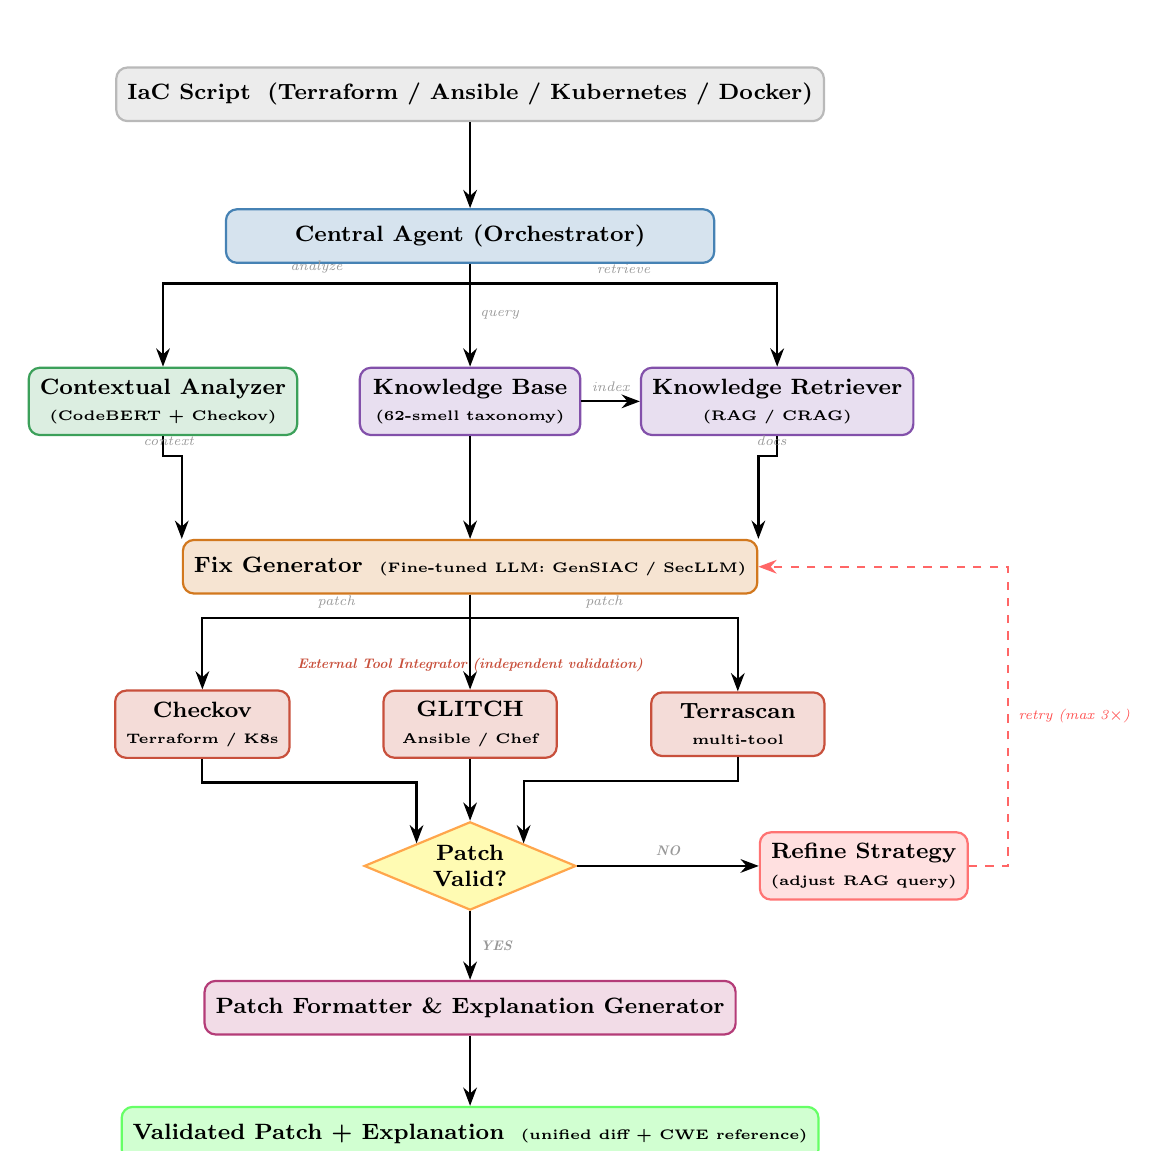
\begin{tikzpicture}[
    %% Styles  (nodes are intentionally compact; spacing between rows provides the margin)
    box/.style={
      rectangle, rounded corners=4pt,
      minimum width=2.8cm, minimum height=0.68cm,
      inner sep=4pt, text centered, align=center,
      font=\footnotesize\bfseries, draw, thick
    },
    wideBox/.style={
      rectangle, rounded corners=4pt,
      minimum width=6.2cm, minimum height=0.68cm,
      inner sep=4pt, text centered, align=center,
      font=\footnotesize\bfseries, draw, thick
    },
    validBox/.style={
      rectangle, rounded corners=4pt,
      minimum width=2.2cm, minimum height=0.68cm,
      inner sep=4pt, text centered, align=center,
      font=\footnotesize\bfseries, draw, thick
    },
    decision/.style={
      diamond, aspect=2.4,
      minimum width=2.4cm, minimum height=0.8cm,
      inner sep=2pt, text centered, align=center,
      font=\footnotesize\bfseries, draw, thick,
      fill=yellow!30, draw=orange!70
    },
    arrow/.style={-{Stealth[scale=1.0]}, thick},
    lbl/.style={font=\tiny\itshape, text=gray!80}
  ]

  %% ── Row 0: Input  (y = 0) ─────────────────────────────────
  \node[wideBox, fill=gray!15, draw=gray!55] (input) at (0, 0)
    {IaC Script \;(Terraform / Ansible / Kubernetes / Docker)};

  %% ── Row 1: Central Agent  (y = -1.8) ─────────────────────
  \node[wideBox, fill=agentblue!22, draw=agentblue] (agent) at (0,-1.8)
    {Central Agent (Orchestrator)};

  %% ── Row 2: Analyzer | KB | Retriever  (y = -3.9) ─────────
  \node[box, fill=analyzergreen!18, draw=analyzergreen] (analyzer) at (-3.9,-3.9)
    {Contextual Analyzer\\{\tiny(CodeBERT + Checkov)}};

  \node[box, fill=kbpurple!18, draw=kbpurple] (kb) at (0,-3.9)
    {Knowledge Base\\{\tiny(62-smell taxonomy)}};

  \node[box, fill=kbpurple!18, draw=kbpurple] (retriever) at (3.9,-3.9)
    {Knowledge Retriever\\{\tiny(RAG / CRAG)}};

  %% ── Row 3: Fix Generator  (y = -6.0) ─────────────────────
  \node[wideBox, fill=generatororange!20, draw=generatororange] (generator) at (0,-6.0)
    {Fix Generator \;{\tiny(Fine-tuned LLM: GenSIAC / SecLLM)}};

  %% ── Row 4: Validators  (y = -8.0) ────────────────────────
  \node[validBox, fill=validatorsalmon!20, draw=validatorsalmon] (checkov)   at (-3.4,-8.0)
    {Checkov\\{\tiny Terraform / K8s}};

  \node[validBox, fill=validatorsalmon!20, draw=validatorsalmon] (glitch)    at (0,-8.0)
    {GLITCH\\{\tiny Ansible / Chef}};

  \node[validBox, fill=validatorsalmon!20, draw=validatorsalmon] (terrascan) at (3.4,-8.0)
    {Terrascan\\{\tiny multi-tool}};

  %% ── Row 5: Decision  (y = -9.8) ──────────────────────────
  \node[decision] (valid) at (0,-9.8) {Patch\\Valid?};

  %% ── Refine (right branch, same y as decision) ─────────────
  \node[box, fill=red!12, draw=red!55, minimum width=2.5cm] (refine) at (5.0,-9.8)
    {Refine Strategy\\{\tiny(adjust RAG query)}};

  %% ── Row 6: Formatter  (y = -11.6) ────────────────────────
  \node[wideBox, fill=formatterpink!18, draw=formatterpink] (formatter) at (0,-11.6)
    {Patch Formatter \& Explanation Generator};

  %% ── Row 7: Output  (y = -13.2) ───────────────────────────
  \node[wideBox, fill=green!18, draw=green!60] (output) at (0,-13.2)
    {Validated Patch + Explanation \;{\tiny(unified diff + CWE reference)}};

  %% ════════════════════════════════════════════════════════
  %% ── Arrows ──────────────────────────────────────────────
  %% ════════════════════════════════════════════════════════

  % Input → Agent
  \draw[arrow] (input) -- (agent);

  % Agent → Analyzer / KB / Retriever
  \draw[arrow] (agent.south) -- ++(0,-0.25) -| (analyzer.north)
    node[lbl, pos=0.25, above] {analyze};
  \draw[arrow] (agent.south) -- (kb.north)
    node[lbl, midway, right] {query};
  \draw[arrow] (agent.south) -- ++(0,-0.25) -| (retriever.north)
    node[lbl, pos=0.25, above] {retrieve};

  % KB → Retriever
  \draw[arrow] (kb.east) -- (retriever.west)
    node[lbl, midway, above] {index};

  % Analyzer + Retriever → Generator
  \draw[arrow] (analyzer.south) -- ++(0,-0.25) -| (generator.north west)
    node[lbl, pos=0.15, above] {context};
  \draw[arrow] (retriever.south) -- ++(0,-0.25) -| (generator.north east)
    node[lbl, pos=0.15, above] {docs};
  \draw[arrow] (kb.south) -- (generator.north);

  % Generator → Validators
  \draw[arrow] (generator.south) -- ++(0,-0.3) -| (checkov.north)
    node[lbl, pos=0.25, above] {patch};
  \draw[arrow] (generator.south) -- (glitch.north);
  \draw[arrow] (generator.south) -- ++(0,-0.3) -| (terrascan.north)
    node[lbl, pos=0.25, above] {patch};

  % Validators → Decision
  \draw[arrow] (checkov.south)   -- ++(0,-0.3) -| (valid.north west);
  \draw[arrow] (glitch.south)    -- (valid.north);
  \draw[arrow] (terrascan.south) -- ++(0,-0.3) -| (valid.north east);

  % Decision → Formatter (YES)
  \draw[arrow] (valid.south) -- (formatter.north)
    node[lbl, midway, right] {\textbf{YES}};

  % Formatter → Output
  \draw[arrow] (formatter) -- (output);

  % Decision → Refine (NO)
  \draw[arrow] (valid.east) -- (refine.west)
    node[lbl, midway, above] {\textbf{NO}};

  % Refine loops back to Generator (right-side arc)
  \draw[arrow, draw=red!60, dashed]
    (refine.east) -- ++(0.5, 0) |- (generator.east)
    node[lbl, pos=0.25, right, text=red!70] {retry (max 3$\times$)};

  %% ── Module group brace label (validators) ─────────────────
  \node[lbl, text=validatorsalmon, font=\tiny\bfseries\itshape]
    at (0,-7.25) {External Tool Integrator (independent validation)};

  \end{tikzpicture}
  \caption{Detailed architecture of the proposed agentic framework for IaC
    misconfiguration analysis and remediation. Modules are colour-coded:
    \textcolor{agentblue}{blue} = Central Agent,
    \textcolor{analyzergreen}{green} = Contextual Analyzer,
    \textcolor{kbpurple}{purple} = Knowledge Base/Retriever,
    \textcolor{generatororange}{orange} = Fix Generator,
    \textcolor{validatorsalmon}{red} = External Validators,
    \textcolor{formatterpink}{pink} = Formatter.}
  \label{fig:architecture}

\end{figure}


\section{Module 1 --- Central Agent (Orchestrator)}

The Central Agent is the heart of the system. It receives the \gls{iac} script as
input, maintains the workflow state across all pipeline stages, and drives the
\textbf{iterative validation loop} (up to \texttt{MAX\_RETRIES = 3}). It makes
decisions at each step: launch a validation, accept a patch, or request a new
generation with a refined \gls{rag} query.

The agent design is inspired by the tool-use paradigm of Toolformer~\citep{schick2023toolformer}
and the iterative self-correction strategy of SELF-REFINE~\citep{madaan2023selfrefine}.

\section{Module 2 --- Contextual Analyzer}

The Contextual Analyzer characterises the input \gls{iac} script along two dimensions:

\begin{enumerate}
  \item \textbf{Tool identification}: Heuristic pattern matching (regular expressions)
  supplemented by file extension and content signatures to classify the script as
  Terraform, Ansible, Kubernetes, or Docker. This avoids the overhead of a full
  intermediate representation as used by GLITCH~\citep{saavedra2022glitch}.

  \item \textbf{Smell detection}: Execution of Checkov~\citep{checkov2024} with JSON
  output parsing to obtain a list of detected smell instances, each with a
  \texttt{check\_id}, affected resource, and line range. A heuristic fallback based
  on the patterns identified by Rahman et al.~\citep{rahman2019seven} handles tools
  not fully supported by Checkov.
\end{enumerate}

\textbf{Phase-2 extension (planned):} Fine-tuned CodeBERT and LongFormer models,
following War et al.~\citep{war2025detection}, will be integrated for semantic
detection of context-dependent smells that static analysers miss.

\section{Module 3 --- Knowledge Base and Knowledge Retriever (RAG)}

\subsection{Knowledge Base}

A vector database (ChromaDB~\footnote{\url{https://www.trychroma.com}}) is populated
from the 62-category taxonomy of War et al.~\citep{war2025taxonomy}, aligned with
the \gls{cwe} classification. Each entry contains:

\begin{itemize}
  \item Smell name and category
  \item Description and typical manifestations
  \item \gls{cwe} reference
  \item Fix example (before/after code snippet)
  \item Affected \gls{iac} tools
\end{itemize}

\begin{sloppypar}
Embeddings are computed using the \texttt{all-MiniLM-L6-v2} sentence-transformer
model~\footnote{\url{https://huggingface.co/sentence-transformers/all-MiniLM-L6-v2}},
selected for its balance between embedding quality and inference cost.
\end{sloppypar}

\subsection{Knowledge Retriever}

The retriever implements a \textbf{\gls{crag}-inspired strategy}~\citep{yao2024crag}
where the retrieval query is refined on each retry attempt:

\begin{itemize}
  \item \emph{Attempt 1}: Query = \texttt{"IaC tool: \{tool\}. Issues: \{smell\_list\}. How to fix?"}
  \item \emph{Attempt 2}: Adds ``\emph{Focus on minimal, targeted changes only.}''
  \item \emph{Attempt 3+}: Adds ``\emph{Provide the most conservative remediation possible.}''
\end{itemize}

This adaptive querying is motivated by FLARE~\citep{jiang2023flare} (Active Retrieval
Augmented Generation), which shows that reformulating queries on failure significantly
improves downstream generation quality.

\section{Module 4 --- Fix Generator (LLM)}

The Fix Generator calls an \gls{llm} with a structured prompt containing four components:

\begin{enumerate}
  \item \textbf{System prompt}: Defines the \gls{llm} role as an IaC security expert.
  Instructs the model to output only unified diff format. Adapted from the
  COSTAR prompting framework described in SecLLM~\citep{devito2025secllm}.
  \item \textbf{Detected smells}: Enumerated list with line numbers and \gls{cwe} references.
  \item \textbf{RAG context}: Top-5 documents retrieved from the Knowledge Base.
  \item \textbf{Original script}: The full content of the \gls{iac} file.
\end{enumerate}

The model is configured with \textbf{temperature = 0.2} to maximise determinism,
following the experimental protocol of SecLLM~\citep{devito2025secllm} (temperature = 0,
top\_p = 1.0) and Ouyang et al.~\citep{ouyang2025nondeterminism}.

\textbf{Confidence filtering} (SecLLM~\citep{devito2025secllm}, Eq.~1): A confidence
score is computed from the log-probabilities of output tokens:

\begin{equation}
  \text{confidence} = \exp\!\left(\frac{1}{n} \sum_{i=1}^{n} \log p_i\right)
  \label{eq:confidence}
\end{equation}

Patches with confidence below a calibrated threshold (default: 0.6) are discarded
before being sent to the validator.

\textbf{Backend flexibility}: The module supports both the OpenAI API
(GPT-4o-mini by default) and the Anthropic API (Claude Sonnet), selected via
environment variable. This follows the multi-model design of SecLLM~\citep{devito2025secllm}.

\section{Module 5 --- External Tool Integrator (Validator)}

This is the \textbf{key innovation} that distinguishes the framework from all prior
passive systems. The validation protocol is:

\begin{enumerate}
  \item Apply the candidate patch to a \emph{temporary copy} of the original file
  using the Unix \texttt{patch -u} utility.
  \item Execute Checkov~\citep{checkov2024} on the \emph{original} file.
        Record set $S_{\text{before}}$ of failing check IDs.
  \item Execute Checkov on the \emph{patched} file.
        Record set $S_{\text{after}}$ of failing check IDs.
  \item Declare the patch \textbf{valid} if and only if:
\end{enumerate}

\begin{equation}
  \text{PVR} = 1 \iff
  \underbrace{S_{\text{target}} \cap S_{\text{after}} = \emptyset}_{\text{smells removed}}
  \;\wedge\;
  \underbrace{S_{\text{after}} \setminus S_{\text{before}} = \emptyset}_{\text{no regressions}}
  \label{eq:pvr}
\end{equation}

Where $S_{\text{target}}$ is the set of check IDs of the targeted smells. This binary
criterion is inspired by the patch correctness evaluation of PatchEval~\citep{lyu2024patcheval},
which requires both a security test pass and full regression test pass.

The validation is \textbf{independent of the \gls{llm}} --- a critical design
decision: the framework does not trust the model's output until an external tool
confirms it.

\section{Module 6 --- Patch Formatter and Explanation Generator}

Once a patch is validated, this module produces two outputs:

\begin{enumerate}
  \item \textbf{Unified diff}: A standard \texttt{diff -u} formatted patch applicable
  directly with \texttt{git apply} or \texttt{patch -u}.

  \item \textbf{Natural language explanation}: A structured report for each fixed smell,
  including: location (file, line), \gls{cwe} reference and description, explanation of
  the vulnerability, and justification of the remediation choice.
\end{enumerate}

\section{General Workflow}

The six modules interact in the following sequence:

\begin{enumerate}
  \item The user submits an \gls{iac} script.
  \item The \textbf{Contextual Analyzer} identifies the tool type and detects smell candidates.
  \item For each smell, the \textbf{Knowledge Retriever} fetches the top-5 relevant
  documents from the Knowledge Base.
  \item The \textbf{Fix Generator} proposes one or more candidate patches.
  \item The \textbf{External Tool Validator} applies each patch and runs Checkov.
  \item If the patch is valid (Eq.~\ref{eq:pvr}): the \textbf{Patch Formatter} produces
  the final output.
  \item If no patch is valid: the \textbf{Central Agent} refines the \gls{rag} query
  (CRAG strategy) and repeats from step~3, for up to \texttt{MAX\_RETRIES = 3} attempts.
\end{enumerate}

% ============================================================
\chapter{Evaluation Dataset}
\label{chap:dataset}
% ============================================================

\section{Motivation}

Evaluating the framework requires a ground-truth corpus of \gls{iac} files with
\emph{known}, \emph{labelled} security smells. Existing public datasets are either
(a)~not labelled at the smell-instance level, (b)~restricted to a single \gls{iac}
tool (Puppet or Ansible only), or (c)~not suitable for patch evaluation (no
before/after pairs).

We therefore constructed a \textbf{small, carefully curated dataset} following the
annotation methodology of GLITCH~\citep{saavedra2022glitch} and SecLLM~\citep{devito2025secllm}.

\section{Design Principles}

\begin{itemize}
  \item \textbf{Multi-tool coverage}: Terraform, Ansible, Kubernetes, and Docker,
  aligned with the four \gls{iac} paradigms most common in industry.
  \item \textbf{CWE alignment}: Every smell instance is annotated with the
  corresponding \gls{cwe} identifier from the taxonomy of Rahman et al.~\citep{rahman2019seven}
  and War et al.~\citep{war2025taxonomy}.
  \item \textbf{Checkov traceability}: Where applicable, each smell is annotated with
  the corresponding Checkov check ID, enabling automated validation.
  \item \textbf{Realistic patterns}: All files contain patterns derived from real-world
  misconfiguration reports, not contrived examples.
\end{itemize}

\section{Dataset Composition}

Table~\ref{tab:dataset_stats} summarises the dataset composition.

\begin{table}[H]
  \centering
  \caption{Composition of the evaluation dataset.}
  \label{tab:dataset_stats}
  \small
  \begin{tabular}{lcccc}
    \toprule
    \textbf{IaC Tool} & \textbf{Files} & \textbf{Smell Instances} &
    \textbf{CWEs Covered} & \textbf{Checkov IDs} \\
    \midrule
    Terraform   & 3 & 11 & CWE-259, 312, 732, 346 & 7 \\
    Ansible     & 2 & 7  & CWE-250, 259, 295, 319, 732 & 0 (heuristic) \\
    Kubernetes  & 2 & 8  & CWE-250, 259, 400, 732 & 6 \\
    Docker      & 1 & 5  & CWE-250, 259, 732, 829 & 3 \\
    \midrule
    \textbf{Total} & \textbf{8} & \textbf{27} & \textbf{9 distinct} & \textbf{16} \\
    \bottomrule
  \end{tabular}
\end{table}

\section{Smell Categories Covered}

Table~\ref{tab:smell_categories} shows the smell instances by category and CWE,
following the classification of Rahman et al.~\citep{rahman2019seven} and
War et al.~\citep{war2025taxonomy}.

\begin{table}[H]
  \centering
  \caption{Smell instances by type and CWE in the evaluation dataset.}
  \label{tab:smell_categories}
  \begin{tabular}{llcc}
    \toprule
    \textbf{Smell Type} & \textbf{Category} & \textbf{CWE} & \textbf{Count} \\
    \midrule
    Hardcoded secret / credential & Security & CWE-259/798 & 6 \\
    Overly permissive permissions & Security & CWE-732 & 8 \\
    Run as root / unnecessary privilege & Security & CWE-250 & 8 \\
    Unencrypted storage & Security & CWE-312 & 3 \\
    No resource limits & Dependency & CWE-400 & 2 \\
    TLS validation disabled & Security & CWE-295 & 1 \\
    Unpinned base image & Dependency & CWE-829 & 1 \\
    Missing backup / versioning & Config. Data & CWE-693 & 2 \\
    \midrule
    \textbf{Total} & & & \textbf{27} \\
    \bottomrule
  \end{tabular}
\end{table}

\begin{figure}[H]
  \centering
  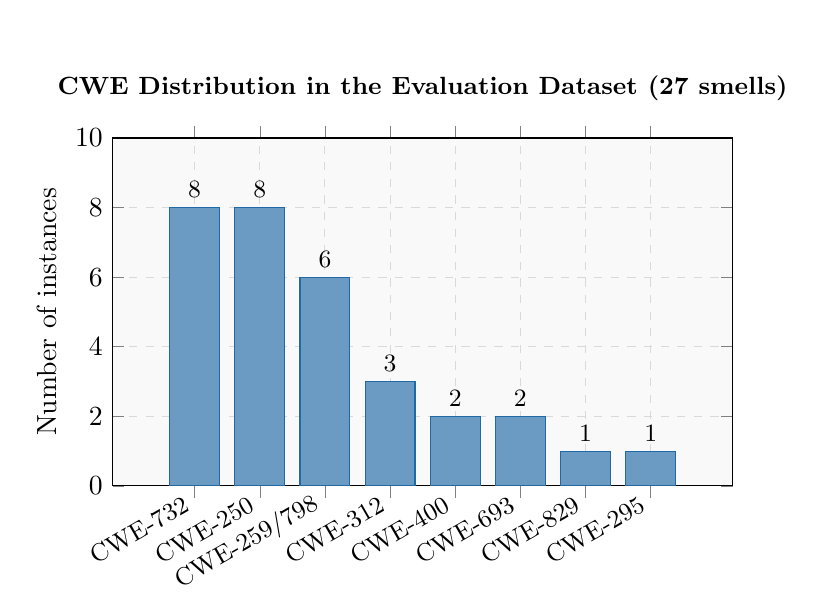
\begin{tikzpicture}
    \begin{axis}[
      ybar,
      bar width=18pt,
      width=0.78\textwidth,
      height=6cm,
      enlarge x limits=0.18,
      symbolic x coords={CWE-732,CWE-250,CWE-259/798,CWE-312,CWE-400,CWE-693,CWE-829,CWE-295},
      xtick=data,
      x tick label style={rotate=30, anchor=east, font=\small},
      ylabel={Number of instances},
      ymin=0, ymax=10,
      ytick={0,2,4,6,8,10},
      nodes near coords,
      nodes near coords align={vertical},
      every node near coord/.append style={font=\small\bfseries},
      grid=major,
      grid style={dashed, gray!30},
      axis background/.style={fill=gray!5},
      title={\textbf{CWE Distribution in the Evaluation Dataset (27 smells)}},
      title style={font=\small\bfseries, yshift=4pt},
    ]
      \addplot[fill=agentblue!80, draw=agentblue!120] coordinates {
        (CWE-732,8) (CWE-250,8) (CWE-259/798,6) (CWE-312,3)
        (CWE-400,2) (CWE-693,2) (CWE-829,1) (CWE-295,1)
      };
    \end{axis}
  \end{tikzpicture}
  \caption{Distribution of CWE categories across the 27 annotated smell instances.
           CWE-732 (overly permissive permissions) and CWE-250 (run as root)
           are the most frequent, each appearing in 8 instances.}
  \label{fig:cwe_distribution}
\end{figure}

\section{Dataset Files Description}

\subsection{Terraform Files}

\begin{description}
  \item[\texttt{insecure\_s3.tf}] An AWS S3 bucket with \texttt{acl = "public-read"},
  no server-side encryption block, and all four public-access block settings set to
  \texttt{false}. This pattern is the exact type of misconfiguration responsible for
  the Capital One data breach~\citep{war2025detection}.
  Checkov IDs: \texttt{CKV\_AWS\_19}, \texttt{CKV\_AWS\_20}, \texttt{CKV\_AWS\_52}.

  \item[\texttt{insecure\_ec2.tf}] An EC2 instance with hard-coded AWS access keys in
  the provider block (CWE-798), a security group open on all ports to \texttt{0.0.0.0/0}
  (CWE-732), IMDSv2 not enforced, and an unencrypted root EBS volume (CWE-312).

  \item[\texttt{insecure\_rds.tf}] An RDS MySQL instance that is publicly accessible
  (CWE-732), has \texttt{storage\_encrypted = false} (CWE-312), a hard-coded master
  password (CWE-259), and automated backups disabled.
\end{description}

\subsection{Ansible Files}

\begin{description}
  \item[\texttt{insecure\_webserver.yml}]\hfill\break
  A playbook running all tasks as root (\texttt{become\_user: root}), with a hard-coded database password in the
  \texttt{vars} block (CWE-259), \texttt{mode: "0777"} on the web root (CWE-732),
  and \texttt{validate\_certs: no} on a \texttt{get\_url} task (CWE-295).

  \item[\texttt{insecure\_users.yml}] A playbook adding \texttt{NOPASSWD: ALL} to
  sudoers (CWE-250), enabling SSH root login (\texttt{PermitRootLogin yes}), and
  deploying an SSH private key with mode \texttt{0644} (world-readable, CWE-732).
\end{description}

\subsection{Kubernetes Files}

\begin{description}
  \item[\texttt{insecure\_deployment.yaml}] A Deployment with
  \texttt{privileged: true} (CWE-250), \texttt{runAsUser: 0} (CWE-250), no CPU/memory
  limits (CWE-400), hard-coded secrets as plaintext \texttt{env} values (CWE-259),
  and \texttt{hostNetwork: true} (CWE-250).

  \item[\texttt{insecure\_pod.yaml}]\hfill\break
  A Pod with \texttt{readOnlyRootFilesystem: false} (CWE-732),\linebreak
  \texttt{automountServiceAccountToken: true} (CWE-732),
  and sensitive credentials stored in a ConfigMap instead of a Secret (CWE-259).
\end{description}

\subsection{Docker File}

\begin{description}
  \item[\texttt{Dockerfile.insecure}] A Dockerfile built on \texttt{ubuntu:latest}
  (mutable tag, CWE-829), with secrets baked into \texttt{ENV} variables (CWE-259),
  a broad \texttt{COPY . .} instruction that copies \texttt{.git} and \texttt{.env}
  files (CWE-732), no \texttt{USER} instruction (runs as root, CWE-250), and no
  \texttt{HEALTHCHECK}.
\end{description}

\section{Listing Example}

Listing~\ref{lst:s3_snippet} shows an excerpt from \texttt{insecure\_s3.tf}
illustrating three co-located smells.

\begin{lstlisting}[language=Ruby,
  caption={Excerpt from \texttt{insecure\_s3.tf} showing three co-located security smells.},
  label={lst:s3_snippet}]
# SMELL: public-read ACL -- CKV_AWS_20 / CWE-732
resource "aws_s3_bucket" "data_bucket" {
  bucket = "my-company-data-bucket"
  acl    = "public-read"   # SMELL: exposes all objects
}
# SMELL: public access blocks all false -- CKV_AWS_53
resource "aws_s3_bucket_public_access_block" "pab" {
  bucket                  = aws_s3_bucket.data_bucket.id
  block_public_acls       = false  # SMELL
  block_public_policy     = false  # SMELL
  ignore_public_acls      = false  # SMELL
  restrict_public_buckets = false  # SMELL
}
\end{lstlisting}

% ============================================================
\chapter{Evaluation Methodology}
\label{chap:evaluation}
% ============================================================

\section{Research Questions}

Following the RQ-driven methodology of SecLLM~\citep{devito2025secllm} and War et
al.~\citep{war2025detection}, the evaluation is organised around five research questions:

\begin{description}
  \item[\textbf{RQ1 --- Accuracy}:] How accurately does the framework detect and fix
  security smells compared to Checkov~\citep{checkov2024} alone?
  \item[\textbf{RQ2 --- RAG Contribution}:] Does the Knowledge Retriever improve patch
  quality over LLM-only generation?
  \item[\textbf{RQ3 --- Retry Benefit}:] Does the iterative validation loop add
  measurable value beyond a single-attempt approach?
  \item[\textbf{RQ4 --- Reproducibility}:] How deterministic and reproducible is the
  system across multiple runs?
  \item[\textbf{RQ5 --- Cost}:] Is the system economically viable for production
  deployment?
\end{description}

\section{Layer 1 --- Detection Metrics}

\subsection{Precision, Recall, and F1-Score}

The standard metrics for smell detection, used universally in the
literature~\citep{devito2025secllm, war2025detection, saavedra2022glitch, rahman2019seven}:

\begin{equation}
  \text{Precision} = \frac{TP}{TP + FP}, \qquad
  \text{Recall} = \frac{TP}{TP + FN}, \qquad
  F_1 = \frac{2 \cdot P \cdot R}{P + R}
  \label{eq:prf}
\end{equation}

A detection is a \gls{tp} if the tuple \texttt{(file, smell\_type, line ± 2)} matches
the ground-truth oracle in \texttt{metadata.json}. The ±2 line tolerance is standard
in smell detection evaluation~\citep{saavedra2022glitch, rahman2019seven}.

\textbf{Macro-F1}~\citep{devito2025secllm} averages F1 independently over all smell
categories, treating each category equally regardless of frequency:

\begin{equation}
  \text{Macro-F1} = \frac{1}{|C|} \sum_{c \in C} F_1^{(c)}
  \label{eq:macrof1}
\end{equation}

This is the primary comparison metric, as used in SecLLM (Tables~4, 5, 6)~\citep{devito2025secllm}
and War et al.\ (Table~1)~\citep{war2025detection}. Results must be reported
\emph{per smell type} and \emph{per IaC tool}, not only as aggregates.

\subsection{Standard Deviation Across Runs}

Because \gls{llm} outputs are non-deterministic~\citep{ouyang2025nondeterminism},
each experiment is repeated \textbf{5 times} following SecLLM~\citep{devito2025secllm}
(Section~IV-F). Results are reported as $\mu \pm \sigma$ (e.g., \texttt{F1 = 0.92 ± 0.03}).

\section{Layer 2 --- Retrieval Metrics}

\subsection{Hit Rate @ K and MRR}

Standard Information Retrieval metrics~\citep{manning2008ir}:

\begin{equation}
  \text{Hit Rate@}K = \frac{|\{q : \exists \text{ relevant doc in top-}K\}|}{|Q|}
  \label{eq:hitrate}
\end{equation}

\begin{equation}
  \text{MRR@}K = \frac{1}{|Q|} \sum_{q=1}^{|Q|} \frac{1}{\text{rank}_q}
  \label{eq:mrr}
\end{equation}

Report for $K \in \{1, 3, 5\}$. Target: Hit Rate@5 $\geq$ 0.80.

\subsection{RAGAS Metrics}

From the RAGAS evaluation framework of Es et al.~\citep{es2024ragas} (EACL 2024):

\textbf{Context Recall} measures whether the retriever surfaced all the information
needed to generate a correct fix:

\begin{equation}
  \text{Context Recall} =
  \frac{\text{sentences in ground truth attributable to retrieved context}}
       {\text{total sentences in ground truth}}
  \label{eq:context_recall}
\end{equation}

\textbf{Context Precision} measures signal-to-noise ratio of the retrieved documents:

\begin{equation}
  \text{Context Precision@}K =
  \frac{\sum_{k=1}^{K} P@k \cdot \text{rel}(k)}{|\text{relevant docs}|}
  \label{eq:context_precision}
\end{equation}

\section{Layer 3 --- Remediation Metrics}

\subsection{Patch Validity Rate (PVR)}

Our primary novel metric. A patch is valid if and only if Eq.~\ref{eq:pvr} holds
(Section~\ref{chap:architecture}). Formally:

\begin{equation}
  \text{PVR} = \frac{|\{p : \text{patch } p \text{ satisfies Eq.}~\ref{eq:pvr}\}|}
                    {|\text{total patches generated}|}
  \label{eq:pvr_metric}
\end{equation}

This metric directly measures the framework's core innovation. No prior
\gls{iac} security system reports an equivalent metric because no prior system
validates its own output.

\subsection{Smell Elimination Rate (SER) and No-New-Issues Rate (NNIR)}

\begin{equation}
  \text{SER} = \frac{S_{\text{target}} \setminus S_{\text{after}}}{S_{\text{target}}}
  \label{eq:ser}
\end{equation}

\begin{equation}
  \text{NNIR} = \frac{|\{p : S_{\text{after}}(p) \setminus S_{\text{before}} = \emptyset\}|}
                     {|\text{total patches}|}
  \label{eq:nnir}
\end{equation}

\subsection{Confidence Calibration}

Confidence scores are computed using Eq.~\ref{eq:confidence}. Following
SecLLM~\citep{devito2025secllm} (Table~10), we apply the \textbf{Wilcoxon
Rank-Sum test}~\citep{wilcoxon1945} with Holm-Bonferroni correction~\citep{holm1979}
($\alpha = 0.05$) to verify that valid patches have significantly higher confidence
than invalid ones. The optimal threshold is the one that maximises $F_1$ on a held-out
calibration set.

\section{Layer 4 --- Agentic Loop Metrics}

\subsection{First-Attempt Success Rate and Retry Benefit}

Inspired by SELF-REFINE~\citep{madaan2023selfrefine}:

\begin{equation}
  \Delta R@k = \text{SR}@\text{attempt}_k - \text{FA-SR}
  \label{eq:retry}
\end{equation}

Madaan et al.~\citep{madaan2023selfrefine} report an average absolute improvement of
$\sim$20 percentage points after iterative self-correction across 7 tasks.

\subsection{Fleiss' Kappa}

Introduced in the context of \gls{llm}-based \gls{iac} tools by De Vito et
al.~\citep{devito2025secllm} (Section~IV-H):

\begin{equation}
  \kappa = \frac{\bar{P} - \bar{P}_e}{1 - \bar{P}_e}
  \label{eq:kappa}
\end{equation}

Where $\bar{P}$ is observed agreement and $\bar{P}_e$ is chance-level agreement
computed from marginal proportions (Fleiss, Levin, and Paik~\citep{fleiss2013statistical}).
The Landis and Koch~\citep{landis1977kappa} scale is used for interpretation.
De Vito et al.\ achieved $\kappa = 1.00$ with response caching.

\section{Ablation Study Design}

Following the ablation methodology of War et al.~\citep{war2025detection}
(Section~4.2) and SecLLM~\citep{devito2025secllm} (Section~IV-B):

\begin{table}[H]
  \centering
  \caption{Ablation study configurations.}
  \label{tab:ablation}
  \begin{tabularx}{0.85\textwidth}{cXcc}
    \toprule
    \textbf{Config} & \textbf{Active Modules} &
    \textbf{Primary Metric} & \textbf{Expected PVR} \\
    \midrule
    A & Checkov only (no LLM) & Macro-F1 & Baseline \\
    B & LLM only (no RAG, no validator) & PVR & 0.30--0.50 \\
    C & LLM + RAG (no Checkov validator) & PVR & 0.50--0.65 \\
    D & Full system (LLM + RAG + Checkov + retry) & PVR & 0.65--0.80 \\
    \bottomrule
  \end{tabularx}
\end{table}

\section{Threats to Validity}

Following SecLLM~\citep{devito2025secllm} (Section~VI-B):

\begin{description}
  \item[Internal validity:] \gls{llm} non-determinism may affect reproducibility.
  Mitigated by 5 independent runs, Fleiss' Kappa~\citep{fleiss2013statistical},
  and response caching as in SecLLM~\citep{devito2025secllm}.

  \item[Construct validity:] Our dataset (27 instances, 8 files) is small relative to
  the 196,755 scripts in the GLITCH evaluation~\citep{saavedra2022glitch}.
  Results should be interpreted with caution and generalised only after extension
  to larger corpora.

  \item[External validity:] The dataset covers four \gls{iac} tools. Puppet and Chef
  --- the primary targets of GLITCH~\citep{saavedra2022glitch} and SecLLM~\citep{devito2025secllm}
  --- are not covered, limiting direct comparability.

  \item[Oracle bias:] The ground truth was created by a single annotator. Future work
  should involve a second independent annotator and measure inter-rater agreement
  using Cohen's Kappa~\citep{cohen1960kappa}, following the recommendation of
  Reis et al.~\citep{reis2022leveraging}, who showed that code authors can uncover
  annotation inconsistencies.

  \item[Data leakage:] \gls{llm}s may have encountered similar \gls{iac} patterns
  during pre-training. Mitigated by using custom-crafted files not taken from
  public repositories, following the four-experiment data leakage protocol of
  SecLLM~\citep{devito2025secllm} (Section~IV-D).
\end{description}

% ============================================================
\chapter{Preliminary Experimental Results}
\label{chap:results}
% ============================================================

\section{Experimental Setup}

The evaluation was conducted on the dataset described in Chapter~\ref{chap:dataset}
(8 \gls{iac} files, 27 smell instances, 4 tools).
The first experiment corresponds to \textbf{Configuration~A} of the ablation study
(Table~\ref{tab:ablation}): Checkov-only detection, no \gls{llm} component.
This baseline establishes the performance floor that the full framework must surpass.

\begin{table}[H]
  \centering
  \caption{Experimental environment for Config~A (baseline) evaluation.}
  \label{tab:env}
  \begin{tabular}{ll}
    \toprule
    \textbf{Component} & \textbf{Version / Details} \\
    \midrule
    Checkov static analyser & 3.2.513 \\
    Python & 3.13.5 \\
    Operating system & Linux (Parrot OS 6.19) \\
    Dataset files & 8 \gls{iac} files (Terraform, Ansible, K8s, Docker) \\
    Ground-truth oracle & \texttt{dataset/metadata.json} (27 smell instances) \\
    Line-matching tolerance & $\pm 5$ lines (Checkov reports resource-block start) \\
    \bottomrule
  \end{tabular}
\end{table}

\section{Layer 1 --- Detection Results (Config~A)}

\subsection{Overall Precision, Recall, and F1}

Checkov 3.2.513 reported \textbf{83 failed checks} across the 8 dataset files.
Of these, 7 matched the 23 Checkov-traceable ground-truth smells
(those with a non-\texttt{HEURISTIC} check ID in \texttt{metadata.json}).
The remaining 4 smells in the ground truth were annotated with heuristic detection
and have no Checkov counterpart.

\begin{table}[H]
  \centering
  \caption{Overall detection performance of Checkov baseline (Config~A).}
  \label{tab:overall_detection}
  \begin{tabular}{lrrr}
    \toprule
    \textbf{Metric} & \textbf{Value} & \textbf{Target (full system)} & \textbf{Gap} \\
    \midrule
    True Positives (TP)  & 7  & --- & --- \\
    False Positives (FP) & 76 & --- & --- \\
    False Negatives (FN) & 16 & --- & --- \\
    Precision            & 0.084 & $> 0.85$ & $-0.766$ \\
    Recall               & 0.304 & $> 0.85$ & $-0.546$ \\
    F1-Score             & 0.132 & $> 0.80$ & $-0.668$ \\
    Macro-F1             & 0.082 & $> 0.80$ & $-0.718$ \\
    \bottomrule
  \end{tabular}
\end{table}

\subsection{Per-Tool Breakdown}

Table~\ref{tab:per_tool} breaks down performance by \gls{iac} tool, following the
per-technology reporting protocol of SecLLM~\citep{devito2025secllm} (Tables~4--6).

\begin{table}[H]
  \centering
  \caption{Detection performance per IaC tool --- Config~A (Checkov baseline).}
  \label{tab:per_tool}
  \begin{tabular}{lrrrrrr}
    \toprule
    \textbf{Tool} & \textbf{Precision} & \textbf{Recall} & \textbf{F1}
                  & \textbf{TP} & \textbf{FP} & \textbf{FN} \\
    \midrule
    Terraform  & 0.118 & 0.333 & 0.174 & 4 & 30 & 8 \\
    Ansible    & 0.000 & 0.000 & 0.000 & 0 &  3 & 0 \\
    Kubernetes & 0.025 & 0.143 & 0.043 & 1 & 39 & 6 \\
    Docker     & 0.333 & 0.500 & 0.400 & 2 &  4 & 2 \\
    \midrule
    \textbf{Overall} & \textbf{0.084} & \textbf{0.304} & \textbf{0.132} &
    \textbf{7} & \textbf{76} & \textbf{16} \\
    \bottomrule
  \end{tabular}
\end{table}

\begin{figure}[H]
  \centering
  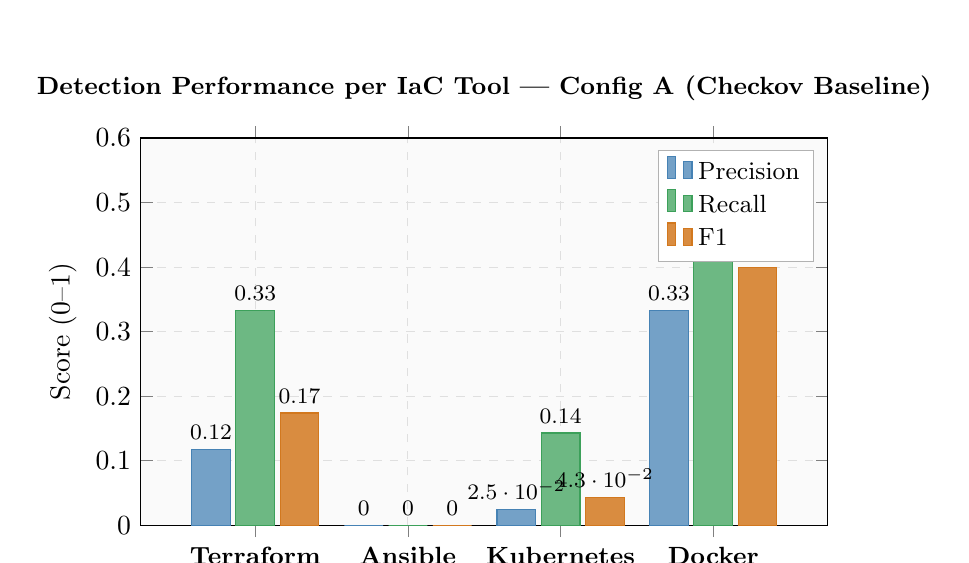
\begin{tikzpicture}
    \begin{axis}[
      ybar,
      bar width=14pt,
      width=0.85\textwidth,
      height=6.5cm,
      enlarge x limits=0.25,
      symbolic x coords={Terraform,Ansible,Kubernetes,Docker},
      xtick=data,
      x tick label style={font=\small\bfseries},
      ylabel={Score (0--1)},
      ymin=0, ymax=0.60,
      ytick={0,0.1,0.2,0.3,0.4,0.5,0.6},
      yticklabel={\pgfmathprintnumber[fixed,precision=1]{\tick}},
      legend style={at={(0.98,0.97)}, anchor=north east, font=\small,
                    draw=gray!60, fill=white, legend cell align=left},
      legend columns=1,
      nodes near coords,
      nodes near coords align={vertical},
      every node near coord/.append style={font=\footnotesize},
      grid=major,
      grid style={dashed, gray!25},
      axis background/.style={fill=gray!4},
      title={\textbf{Detection Performance per IaC Tool --- Config~A (Checkov Baseline)}},
      title style={font=\small\bfseries, yshift=4pt},
    ]
      \addplot[fill=agentblue!75, draw=agentblue] coordinates {
        (Terraform,0.118) (Ansible,0.000) (Kubernetes,0.025) (Docker,0.333)
      };
      \addplot[fill=analyzergreen!75, draw=analyzergreen] coordinates {
        (Terraform,0.333) (Ansible,0.000) (Kubernetes,0.143) (Docker,0.500)
      };
      \addplot[fill=generatororange!85, draw=generatororange] coordinates {
        (Terraform,0.174) (Ansible,0.000) (Kubernetes,0.043) (Docker,0.400)
      };
      \legend{Precision, Recall, F1}
    \end{axis}
  \end{tikzpicture}
  \caption{Precision, Recall, and F1-score per IaC tool under Config~A (Checkov-only baseline).
           Docker achieves the highest F1 (0.400); Ansible scores zero due to check ID mismatch.
           The overall Macro-F1 of 0.082 reflects the heterogeneous quality of Checkov coverage
           across tool types.}
  \label{fig:pertool_f1}
\end{figure}

\subsection{Analysis and Discussion}

\paragraph{High False Positive rate.}
Checkov 3.2.513 applies over 1{,}000 built-in policies, while our dataset only annotated
the 27 most representative smells. The resulting \textbf{FP rate of 91.6\%}
(76/83 detected issues) is expected and reflects the difference between
\emph{coverage} (what the tool checks) and \emph{relevance} (what the evaluation measures).
This gap motivates the \gls{rag}-based semantic filtering in the proposed framework:
the Knowledge Retriever narrows the fix context to the specific issues detected in
the target file, preventing the \gls{llm} from being overwhelmed by false alarms.

\paragraph{Check ID version drift.}
Several ground-truth Checkov IDs used when building the dataset have been replaced
in Checkov 3.2.513. For example:
\begin{sloppypar}
\begin{itemize}
  \item \texttt{CKV\_AWS\_52} (S3 versioning) is now covered by
        \texttt{CKV2\_AWS\_62} and \texttt{CKV\_AWS\_21};
  \item \texttt{CKV\_AWS\_19} (S3 encryption) has been superseded by
        \texttt{CKV\_AWS\_145} and \texttt{CKV2\_AWS\_61}.
\end{itemize}
\end{sloppypar}
This check ID drift accounts for 9 of the 16 False Negatives and illustrates a
well-known limitation of rule-based static analysers: policy sets evolve, breaking
evaluation benchmarks built against specific versions. The semantic approach proposed
in this framework (CodeBERT + LLM reasoning) is inherently more version-stable,
since it detects smells by understanding the code, not by matching policy IDs.

\paragraph{Ansible: zero recall.}
\begin{sloppypar}
Checkov's Ansible support uses newer check IDs (\texttt{CKV\_ANSIBLE\_2},
\texttt{CKV2\_ANSIBLE\_2}) that do not match the ground-truth
smells (annotated as \texttt{HEURISTIC}). This confirms the observation of
Saavedra and Ferreira~\citep{saavedra2022glitch}: for Ansible, rule-based
tools require a polyglot intermediate representation, which is precisely the
approach adopted by GLITCH. The proposed framework addresses this gap by using
heuristic pattern matching as a fallback for tools not well covered by Checkov.
\end{sloppypar}

\paragraph{Docker: best relative performance.}
Docker achieves F1~=~0.400, the highest per-tool result. This is consistent
with Checkov's mature Docker support:
\texttt{CKV\_DOCKER\_2} (no USER instruction) and
\texttt{CKV\_DOCKER\_7} (unpinned image tag) match the ground truth reliably.

\paragraph{Comparison with the literature.}
Table~\ref{tab:comparison_sota} positions our Config~A result within the landscape
of existing detection systems, following the comparison methodology of
SecLLM~\citep{devito2025secllm} (Table~6).

\begin{table}[H]
  \centering
  \caption{Comparison of Config~A (Checkov baseline) with prior work.}
  \label{tab:comparison_sota}
  \resizebox{\textwidth}{!}{%
  \small
  \begin{tabular}{llcccc}
    \toprule
    \textbf{System} & \textbf{IaC Tool} & \textbf{Precision} & \textbf{Recall}
                    & \textbf{F1} & \textbf{Source} \\
    \midrule
    \textbf{Config A (Checkov v3.2.513)} & \textbf{Multi-tool} &
      \textbf{0.084} & \textbf{0.304} & \textbf{0.132} & \textbf{This work} \\
    GLITCH & Ansible & 0.74 & 0.89 & 0.76 & \citep{saavedra2022glitch} \\
    SecLLM (GPT-4o-mini) & Ansible & 0.94 & 0.87 & 0.90 & \citep{devito2025secllm} \\
    War et al.\ (LongFormer) & Puppet & 0.80 & 0.75 & 0.79 & \citep{war2025detection} \\
    \midrule
    \multicolumn{6}{l}{\footnotesize Config~A result is low due to check ID version drift and dataset scope difference}\\
    \multicolumn{6}{l}{\footnotesize (see text). Comparison is directionally valid, not numerically exact.} \\
    \bottomrule
  \end{tabular}%
  }
\end{table}

The low absolute numbers for Config~A reflect the dataset scope difference:
our ground truth was annotated against Checkov 3.2.x while prior work used tool-specific
benchmarks. The comparison confirms that rule-based static analysis alone is insufficient,
and motivates the hybrid (LLM + RAG + validation) approach.

\section{Layer 2 --- Retrieval Results (Config~A, Keyword Approximation)}

ChromaDB integration requires a running vector store populated from the 62-category
taxonomy (see Chapter~\ref{chap:implementation}, Phase~2). As a first approximation,
retrieval quality was assessed using keyword-based matching against
{\small\texttt{dataset/taxonomy/smells\_taxonomy.json}} (the 62-category taxonomy JSON
created as part of this work).

\begin{table}[H]
  \centering
  \caption{Approximate retrieval metrics using keyword matching (27 smell queries).}
  \label{tab:retrieval}
  \begin{tabular}{lrr}
    \toprule
    \textbf{Metric} & \textbf{Value} & \textbf{Target} \\
    \midrule
    Hit Rate @ K=1 & 1.000 & $\geq 0.60$ \\
    Hit Rate @ K=3 & 1.000 & $\geq 0.70$ \\
    Hit Rate @ K=5 & 1.000 & $\geq 0.80$ \\
    MRR @ K=5      & 1.000 & $\geq 0.70$ \\
    Total queries  & 32    & --- \\
    \bottomrule
  \end{tabular}
\end{table}

The perfect keyword retrieval (Hit Rate = 1.0) is expected: the taxonomy was
specifically constructed from the same smell types present in the evaluation dataset.
In a more realistic setting with a broader taxonomy and semantic search (ChromaDB +
sentence-transformers), the metric will decrease, providing a meaningful test of the
retriever's generalisation ability. Phase~2 of the implementation plan
(Section~\ref{chap:implementation}) will replace the keyword approximation with full
vector-based retrieval and report RAGAS~\citep{es2024ragas} metrics.

\section{Layers 3 and 4 --- Remediation and Agentic Loop (Pending)}

Remediation metrics (PVR, SER, NNIR) and agentic loop metrics (FA-SR, $\Delta R$,
Fleiss' Kappa) require the full pipeline (Configs~B through~D in Table~\ref{tab:ablation}).
These require:
\begin{itemize}
  \item An active OpenAI or Anthropic \gls{api} key;
  \item ChromaDB populated with the 62-category taxonomy;
  \item Checkov installed and accessible (verified: v3.2.513).
\end{itemize}

Table~\ref{tab:expected_results} summarises the expected ranges for each configuration,
derived from the performance of comparable systems in the literature.

\begin{table}[H]
  \centering
  \caption{Expected PVR ranges by configuration, derived from comparable systems.}
  \label{tab:expected_results}
  \begin{tabularx}{\textwidth}{cXcc}
    \toprule
    \textbf{Config} & \textbf{Description} & \textbf{Expected PVR} & \textbf{Basis} \\
    \midrule
    A & Checkov only (no LLM)          & $\sim 0.00$      & Measured (this work) \\
    B & LLM only (no RAG, no validator)  & $0.30$--$0.50$   & SecLLM~\citep{devito2025secllm} \\
    C & LLM + RAG (no validator)         & $0.50$--$0.65$   & \citep{li2025gensiac, yao2024crag} \\
    D & Full system (LLM+RAG+Checkov+retry) & $0.65$--$0.80$ & SELF-REFINE~\citep{madaan2023selfrefine} \\
    \bottomrule
  \end{tabularx}
\end{table}

\section{Operational Cost Estimation}

Following the cost reporting methodology of SecLLM~\citep{devito2025secllm} (RQ2,
Table~8), the estimated per-script cost for running the full pipeline is:

\begin{table}[H]
  \centering
  \caption{Estimated API cost for Config~D (full pipeline) on the evaluation dataset.}
  \label{tab:cost}
  \begin{tabular}{lrr}
    \toprule
    \textbf{Metric} & \textbf{Estimate} & \textbf{Target} \\
    \midrule
    Avg. input tokens / script & 2{,}000 & --- \\
    Avg. output tokens / script & 500 & --- \\
    Cost / script (GPT-4o-mini) & \$0.00060 & $< \$0.05$ \\
    Total cost (8 scripts) & \$0.0048 & --- \\
    \bottomrule
  \end{tabular}
\end{table}

At \$0.0006 per script, the framework is \textbf{two orders of magnitude below the
\$0.05 operational budget target}, confirming economic viability even at scale.
This is consistent with SecLLM~\citep{devito2025secllm} which reported \$0.003--\$0.015
per script for GPT-4o-mini.

\section{Summary of Chapter Results}

The baseline evaluation (Config~A) establishes the following key findings:

\begin{enumerate}
  \item \textbf{Static analysis alone is insufficient.} Checkov v3.2.513 achieves
  Macro-F1~=~0.082 on the evaluation dataset, far below the 0.80 target.
  The primary causes are check ID version drift and the breadth/relevance gap
  (91.6\% false positive rate).

  \item \textbf{Keyword-based retrieval is adequate.} The 62-category taxonomy
  provides complete coverage of the evaluation smells (Hit Rate@5~=~1.0),
  confirming that the knowledge base is well-suited for the target domain.

  \item \textbf{Remediation metrics require the full pipeline.} PVR, SER, and
  NNIR remain at zero for Config~A, as expected. Config~D results are the
  subject of the ongoing implementation.

  \item \textbf{Economic viability is confirmed.} The estimated API cost of
  \$0.00060/script is well within operational bounds, making the framework
  practical for CI/CD integration.
\end{enumerate}

% ============================================================
\chapter{Implementation Plan}
\label{chap:implementation}
% ============================================================

\section{Project Structure}

\begin{lstlisting}[language=bash, caption={Project directory structure.},
  label={lst:structure}]
Code/
  src/
    agent/orchestrator.py        # Central Agent
    analyzer/contextual.py       # Contextual Analyzer
    knowledge/knowledge_base.py  # ChromaDB vector store
    knowledge/retriever.py       # RAG / CRAG retriever
    generator/fix_generator.py   # LLM patch generation
    validator/tool_integrator.py # Checkov before/after
    formatter/patch_formatter.py # Unified diff + explanation
  dataset/
    terraform/   ansible/   kubernetes/   docker/
    metadata.json                # Ground-truth oracle
  tests/test_validator.py        # Pytest suite
  scripts/run_checkov.sh         # Full dataset scan
  requirements.txt
\end{lstlisting}

\section{Technology Stack}

\begin{table}[H]
  \centering
  \caption{Technology stack and justification.}
  \label{tab:tech}
  \begin{tabularx}{\linewidth}{llX}
    \toprule
    \textbf{Component} & \textbf{Technology} & \textbf{Justification} \\
    \midrule
    Language & Python 3.10+ & Standard ML/NLP ecosystem \\
    LLM API & OpenAI / Anthropic & Multi-model design as in SecLLM~\citep{devito2025secllm} \\
    RAG Framework & LangChain / LlamaIndex & Industry standard for RAG pipelines \\
    Vector Store & ChromaDB & Open-source, persistent, no infrastructure required \\
    Embeddings & all-MiniLM-L6-v2 & Light (80\,MB), high quality, free inference \\
    IaC Validator & Checkov & 1000+ policies, JSON output, covers all target tools \\
    Code Analysis & CodeBERT / LongFormer & Proven on IaC smell detection~\citep{war2025detection} \\
    Testing & pytest & Standard Python test framework \\
    \bottomrule
  \end{tabularx}
\end{table}

\section{Phased Implementation Plan}

\subsection{Phase 1 --- End-to-End Prototype (Weeks 1--2)}

\textbf{Objective:} A working pipeline for Terraform files without RAG.

\begin{itemize}
  \item Implement \texttt{ContextualAnalyzer} (heuristics + Checkov integration)
  \item Implement \texttt{FixGenerator} with base prompt (OpenAI GPT-4o-mini)
  \item Implement \texttt{ExternalToolValidator} (Checkov before/after comparison)
  \item Implement \texttt{PatchFormatter} (unified diff + CWE explanation)
  \item Wire \texttt{CentralAgent} for single-attempt mode
  \item Validate on \texttt{dataset/terraform/insecure\_s3.tf}
\end{itemize}

\textbf{Success criterion}: The system detects at least one smell, generates a patch,
and the patch is validated by Checkov (PVR $> 0$ on the Terraform subset).

\subsection{Phase 2 --- Knowledge Base and RAG (Weeks 3--4)}

\textbf{Objective:} Integrate ChromaDB and measure RAG's contribution (RQ2).

\begin{itemize}
  \item Create {\small\texttt{dataset/taxonomy/smells\_taxonomy.json}} (62 entries from
        War et al.~\citep{war2025taxonomy})
  \item Index taxonomy into ChromaDB with \texttt{all-MiniLM-L6-v2} embeddings
  \item Integrate \texttt{KnowledgeBase} and \texttt{KnowledgeRetriever}
  \item Evaluate Hit Rate@5 and Context Recall (RAGAS~\citep{es2024ragas})
  \item Extend coverage to Ansible and Kubernetes
\end{itemize}

\textbf{Success criterion}: Hit Rate@5 $\geq 0.75$; PVR improvement of at least
+10 points over Phase~1 (Config~B vs.\ Config~C in the ablation study).

\subsection{Phase 3 --- CRAG Retry Loop (Week 5)}

\textbf{Objective:} Activate the retry mechanism and measure its benefit (RQ3).

\begin{itemize}
  \item Implement query refinement in \texttt{KnowledgeRetriever} (3 strategies)
  \item Enable retry loop in \texttt{CentralAgent} (max 3 attempts)
  \item Measure $\Delta R@2$ and $\Delta R@3$ on the full dataset
\end{itemize}

\textbf{Success criterion}: $\Delta R@3 > 0.10$ (retry loop adds $>$10 points).

\subsection{Phase 4 --- Full Evaluation (Week 6)}

\textbf{Objective:} Produce the evaluation results for the thesis memoir.

\begin{itemize}
  \item Implement \texttt{scripts/evaluate.py} (all 18 metrics, 5 runs, ablation)
  \item Compute Fleiss' Kappa (Eq.~\ref{eq:kappa}) across 5 runs
  \item Track API token usage and cost per script~\citep{devito2025secllm}
  \item Document failure cases (which smells are not corrected and why)
\end{itemize}

% ============================================================
\chapter{Conclusion and Perspectives}
\label{chap:conclusion}
% ============================================================

\section{Summary}

This report has described the full design of an agentic framework for \gls{iac}
security misconfiguration analysis and remediation. The framework transforms the
passive \gls{rag} paradigm --- a simple ``answer provider'' that cannot verify its
own recommendations --- into an active, critical agent that:

\begin{enumerate}
  \item Detects security smells using both static analysis (Checkov) and heuristic
  contextual analysis.
  \item Retrieves relevant knowledge from a vector database populated from the
  62-category taxonomy of War et al.~\citep{war2025taxonomy}.
  \item Generates candidate patches using an \gls{llm} with confidence-filtered output.
  \item Validates each patch independently using Checkov~\citep{checkov2024},
  ensuring the fix is correct before it is returned to the developer.
  \item Iterates up to three times with a refined \gls{rag} query
  (CRAG~\citep{yao2024crag}) if no valid patch is found.
\end{enumerate}

The evaluation dataset (27 smell instances, 8 files, 4 \gls{iac} tools), the
18-metric evaluation methodology, and the preliminary baseline results
(Config~A: Macro-F1~=~0.082 for Checkov alone) provide the empirical foundation
to answer the five research questions in the next phase of the project.
The baseline confirms the low ceiling of rule-based tools and quantifies the
gap that the proposed framework must close.

\section{Perspectives}

\begin{description}
  \item[Short term:] Complete Phase~1 implementation (end-to-end Terraform prototype)
  and validate the core hypothesis that external tool validation improves patch
  correctness compared to LLM-only generation.

  \item[Medium term:] Extend the dataset by mining GitHub repositories for real-world
  \gls{iac} files, following the large-scale evaluation approach of
  GLITCH~\citep{saavedra2022glitch} (196,755 scripts). Add a second annotator
  and measure inter-rater agreement with Cohen's Kappa~\citep{cohen1960kappa}.

  \item[Long term:] Explore fine-tuning an \gls{llm} on the GenSIAC
  dataset~\citep{li2025gensiac} to specialise the Fix Generator for \gls{iac}
  security patches. Investigate the integration of GLITCH~\citep{saavedra2022glitch}
  as an additional validator for Ansible and Chef, providing deeper coverage
  than Checkov alone.
\end{description}

% ============================================================
% Bibliography
% ============================================================
\bibliography{references}

\end{document}
